 

\chapter{Opis wykorzystywanych narzędzi}
%Rozdział opisuje zastosowanie 

\section{Z3 Solver}
Z3 to wydajny SMT solver dostępny bezpłatnie przez Microsoft Research. Z3 jest solverem dla logiki symbolicznej, będącej podstawą wielu narzędzi inżynierii oprogramowania. Solwery SMT polegają na ścisłej integracji wyspecjalizowanych silników walidacyjnych. Każdy silnik jest elementem ogólnej struktury i implementuje wyspecjalizowane algorytmy. Przykładowo, silnik Z3 dla arytmetyki obejmuje Simplex, cięcia i rozumowanie wielomianowe, podczas gdy silnik dla obsługi ciągów znaków i wyrażeń regularnych korzysta z metod symbolicznych pochodnych języków regularnych. Wspólną cechą wielu algorytmów jest sposób, w jaki wykorzystują dwoistość między znajdowaniem rozwiązań spełniających a dowodów odrzucających. Solver ten integruje również silniki do wnioskowań globalnych i lokalnych oraz globalnej propagacji.
Z3 jest używany w szerokim zakresie zastosowań inżynierii oprogramowania, obejmując weryfikację programów, walidację kompilatorów, testowanie, fuzzing przy użyciu dynamicznego wykonywania symbolicznego, rozwój oprogramowania oparty na modelach, weryfikację sieci i optymalizację.
Z3 może być zbudowany przy użyciu Visual Studio, pliku Makefile lib CMake. Zapewnia obsługę wielu języków programowania, w tym .NET, C, C++, Java, OCaml, Web Assembly i Python.

\subsection{Architektura systemu}
	\begin{figure}
	\centering
	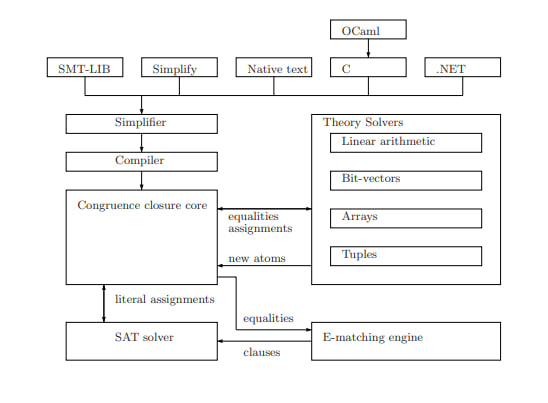
\includegraphics[width=0.7\linewidth]{screenshot001}
	\caption{}
	\label{fig:screenshot001}
\end{figure}
Z3 integruje nowoczesny solver SAT oparty na DPLL, bazowy solwer dla teorii, który obsługuje równości i funkcje nieinterpretowane, specjalistyczne silniki (dla arytmetyki, tablic itp.) oraz maszynę abstrakcyjną E-matching (dla kwantyfikatorów). Z3 jest zaimplementowany w C++. Schematyczny przegląd Z3 pokazano na poniższym rysunku.


\textbf{Simplifier}. Formuły wejściowe są najpierw przetwarzane przy użyciu niekompletnego, ale wydajnego uproszczenia. Simplifier stosuje standardowe zasady redukcji algebraicznej, takie jak $p \land true \implies p$, ale także wykonuje ograniczone uproszczenie kontekstowe, identyfikując definicje równościowe w danym kontekście i redukuje pozostałą formułę przy użyciu definicji, na przykład $x = 4 \land q(x) \implies x = 4 \land q(4)$. Trywialnie spełnialny spójnik $x = 4$ nie jest kompilowany do jądra, ale zachowany poza nim na wypadek, gdyby klient wymagał modelu do obliczenia x.


\section{Yices Solver}
sdcssdsdf

\section{CVC5 Solver}
sdsdcfsdfcdsf